\chapter{Тодорхой интеграл}
Тодорхой интеграл нь бүх шинжлэх ухаанд хамгийн өргөн хэрэглэгддэг 
ойлголт төдийгүй хэрэглээний болон тооцоололын салбарын гол хэрэглэгдэхүүн болдог. Дифференциал тоолол нь танин мэдэхгүйн дедукцийн аргын математик хувилбар бол Тодорхой интеграл нь танин мэдэхгүйн тусгайгаас ерөнхийд шилжих аргын математикийн хувилбар юм. Бид Риманы интегралтай танилцах бөгөөд Риманы интегралаас гадна Лебег болон өөр интегралууд бий.

\section{ Интеграл нийлбэр}
$y=f(x)$ сөрөг бус, тасралтгүй функц $[a,b]$ завсар дээр өгөгдсөн гэж үзье.  $x=a$-аас $x=b$ хүртэлх функцийн график доорх хавтгайн хэсгийн талбайг олох асуудал авч үзье.

\begin{center}
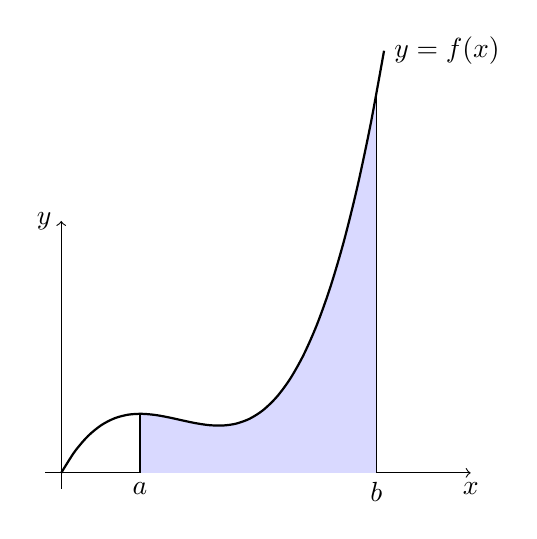
\begin{tikzpicture}[scale=1.0]
  % Axes
  \draw[->] (-0.2,0) -- (5.2,0) node[below] {$x$};
  \draw[->] (0,-0.2) -- (0,3.2) node[left] {$y$};
   \fill[blue!15] (1,0) -- plot[domain=1:4] (\x,{0.15*(2*\x*\x*\x-9*\x*\x+12*\x)}) -- (4,0) -- cycle;

  % Function
  \draw[domain=0:4.1,smooth,thick] plot(\x,{0.15*(2*\x*\x*\x-9*\x*\x+12*\x)}) node[right] {$y=f(x)$};
  % a,b
  \draw (1,0) node[below] {$a$} -- (1,0.75);
  \draw (4,0) node[below] {$b$} -- (4,4.8);
   % Area shading
\end{tikzpicture}
\end{center}
Энэ талбайг тооцоолохын тулд $[a,b]$ завсрыг олон жижиг хэсэгт хувааж,
дөрвөлжин багануудын талбайн нийлбэрээр \emph{ойролцоогоор} үнэлнэ.
\begin{definition}[Хуваалт]
\[
P:\quad a = x_0 < x_1 < \dots < x_n = b
\]
тоонуудын дарааллыг $[a,b]$ завсрын \emph{хуваалт} гэнэ. $[x_{k-1},x_k]$ завсрын уртыг $\Delta x_k$ гэвэл $\Delta x_k = x_k - x_{k-1}$ байна. 
\[
|P| = \max_{1\le k\le n} \Delta x_k
\] тоог $P$ хуваалтын \emph{диаметр} гэнэ.
\end{definition}

 $f$ функцийн $[a,b]$ завсар дээрх графикийн хэсгийн доор орших талбайг ойролцоор үнэлэхийн тулд $[a,b]$ завсарыг $4$ хэсэгт хувааж хуваалтын хэсэг бүрээс $\,\xi_k \in [x_{k-1},x_k]\,$ цэг сонгож $f(\xi_k)$ өндөртэй тэгш өнцөгт баганууд байгуулъя.

\begin{center}
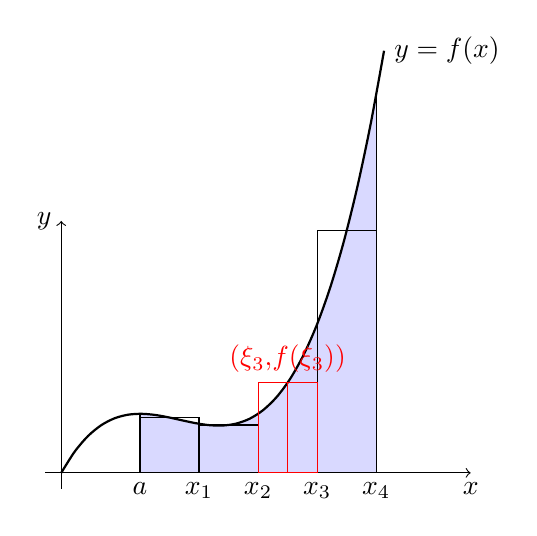
\begin{tikzpicture}[scale=1.0]
  % Axes
  \draw[->] (-0.2,0) -- (5.2,0) node[below] {$x$};
  \draw[->] (0,-0.2) -- (0,3.2) node[left] {$y$};
   \fill[blue!15] (1,0) -- plot[domain=1:4] (\x,{0.15*(2*\x*\x*\x-9*\x*\x+12*\x)}) -- (4,0) -- cycle;

  % a,b
  \draw (1,0) node[below] {$a$} -- (1,0.75);
  \draw (4,0) -- (4,4.8);
  % Partition points
  \def\xa{1}
  \def\xb{4}
  \def\n{4}
  \pgfmathsetmacro{\h}{(\xb-\xa)/\n}
  % Rectangles with right endpoints
  \foreach \k in {1,...,\n}{
    \pgfmathsetmacro{\xkm}{(\xa+(\k-1)*\h)}
    \pgfmathsetmacro{\xk}{\xa+\k*\h}
     \node[below] at (\xk,0) {$x_{\k}$};
    \pgfmathsetmacro{\xkl}{\xa+(\k-0.5)*\h}
    \pgfmathsetmacro{\f}{0.15*(2*\xkl*\xkl*\xkl-9*\xkl*\xkl+12*\xkl)}
    \draw(\xkm,0) rectangle (\xk,\f);
    \draw[dashed] (\xk,0) -- (\xk,\f);
  }

  % Function
  \draw[domain=0:4.1,smooth,thick] plot(\x,{0.15*(2*\x*\x*\x-9*\x*\x+12*\x)}) node[right] {$y=f(x)$};
   \pgfmathsetmacro{\xkl}{2.875}
   \pgfmathsetmacro{\f}{0.15*(2*\xkl*\xkl*\xkl-9*\xkl*\xkl+12*\xkl)}
    \draw[red] (\xkl,0) -- (\xkl,\f) node[above] {($\xi_3$,$f(\xi_3)$)};
    \draw[red](2.5,0) rectangle (3.25,\f);
\end{tikzpicture}
\end{center}

Тэгш өнцөгт багануудын нийт талбай
\[
S(P) = \sum_{k=1}^4 f(\xi_k)\,\Delta x_k,
\] болно. 
\begin{definition}[Интеграл нийлбэр] $y=f(x)$ функцийн хувьд $[a;b]$ завсарын $P$ хуваалтаар 
 \[
S(P) = \sum_{k=1}^n f(\xi_k)\,\Delta x_k,
\] зохиосон нийлбэрийг $y=f(x)$ функцээс $[a;b]$ завсараар авсан \emph{интеграл нийлбэр} гэнэ.
\end{definition}
Дээрх байдлаар талбайг ойролцоо тооцоолохдоо хуваалтыг олон болгож авбал тэгш өнцөгтүүдийн талбайн нийлбэр нь бидний олох талбайн утгаруу дөхнө. 
\begin{center}
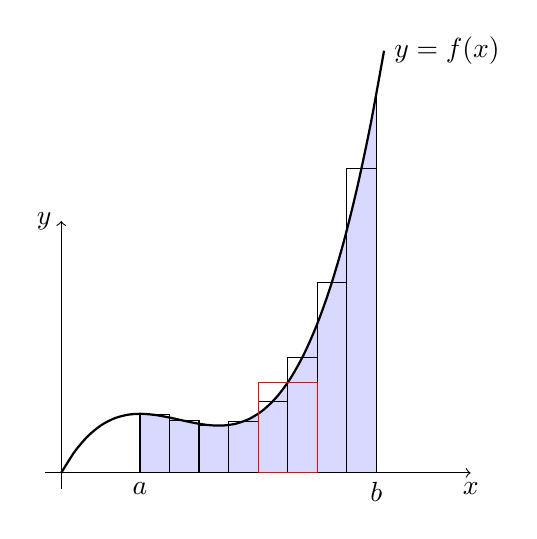
\begin{tikzpicture}[scale=1.0]
  % Axes
  \draw[->] (-0.2,0) -- (5.2,0) node[below] {$x$};
  \draw[->] (0,-0.2) -- (0,3.2) node[left] {$y$};
   \fill[blue!15] (1,0) -- plot[domain=1:4] (\x,{0.15*(2*\x*\x*\x-9*\x*\x+12*\x)}) -- (4,0) -- cycle;

  % a,b
  \draw (1,0) node[below] {$a$} -- (1,0.75);
  \draw (4,0) node[below] {$b$}-- (4,4.8);
  % Partition points
  \def\xa{1}
  \def\xb{4}
  \def\n{8}
  \pgfmathsetmacro{\h}{(\xb-\xa)/\n}
  % Rectangles with right endpoints
  \foreach \k in {1,...,\n}{
    \pgfmathsetmacro{\xkm}{(\xa+(\k-1)*\h)}
    \pgfmathsetmacro{\xk}{\xa+\k*\h}
    \pgfmathsetmacro{\xkl}{\xa+(\k-0.5)*\h}
    \pgfmathsetmacro{\f}{0.15*(2*\xkl*\xkl*\xkl-9*\xkl*\xkl+12*\xkl)}
    \draw(\xkm,0) rectangle (\xk,\f);
    \draw[dashed] (\xk,0) -- (\xk,\f);
  }

  % Function
  \draw[domain=0:4.1,smooth,thick] plot(\x,{0.15*(2*\x*\x*\x-9*\x*\x+12*\x)}) node[right] {$y=f(x)$};
  \pgfmathsetmacro{\xkl}{2.875}
   \pgfmathsetmacro{\f}{0.15*(2*\xkl*\xkl*\xkl-9*\xkl*\xkl+12*\xkl)}
   \draw[red](2.5,0) rectangle (3.25,\f);
\end{tikzpicture}
\end{center}

\section{Тодорхой интегралын тодорхойлолт (Риман)}

\begin{definition}[Тодорхой интеграл]
$f$ функц $[a,b]$ завсар дээр өгөгдсөн байг. Хэрэв
ямар ч хуваалт $P$ болон $[x_{k-1},x_k]$ бүр дээрх дурын $\xi_k\in[x_{k-1},x_k]$–ийн хувьд интеграл нийлбэрүүд
\[
S(P) = \sum_{k=1}^n f(\xi_k)\,\Delta x_k
\]
нь хуваалтын диаметр тэгрүү тэмүүлэхэд тогтмол тоо $I$–рүү дөхдөг, өөрөөр хэлбэл
\[
\lim\limits_{|P|\to 0} S(P)=I
\]
байвал $f$ функцыг $[a,b]$ завсарт \emph{интегралчлагдах функц} гэнэ.
Тэр тохиолдолд $I$–г $f$-ийн $[a;b]$ завсраар авсан  Риманын интеграл гээд
\[
I = \int_a^b f(x)\,dx
\]
хэмээн бичнэ. Цаашид Риманы интеграл эсвэл товчоор тодорхой интеграл гэнэ.
\end{definition}

Ойлгомжтойгоор хэлбэл: хуваалтыг улам нарийсгах тусам интеграл нийлбэрүүд
$I$ тооруу дөхөж байвал тэр $I$ тоог тодорхой интеграл гэнэ. Гэвч тодорхойлолтод дагуу ямар функцийн интеграл оршин байх эсэх тухай хариулт байхгүй байна. Энэ асуултанд дараах теорем хариулт өгнө.  
\begin{theorem}[Тасралтгүй функцийн интегралчлагдах чанар]
Хэрэв $f$ функц $[a,b]$ завсар дээр тасралтгүй бол
$f$ нь $[a,b]$ дээр Риманы утгаар интегралчлагдана.
\end{theorem}

Энэ теоремоос \emph{тасралтгүй} функцүүдийн хувьд тодорхой интеграл заавал оршин байдаг болох нь харагдана. Мөн тасралттай боловч интегралчлагдах функцүүд оршин байна.
\begin{example}
    $\displaystyle \int_0^1 x^2\,dx$–ийг интеграл нийлбэрийн хязгаар бодож тооцоол.

$[0,1]$ завсрыг $n$ тэнцүү хэсэгт хуваая:
\[
x_k = \frac{k}{n},\qquad \Delta x = \frac1n,\qquad k=0,1,\dots,n.
\]
$\xi_k$ цэгүүдийг хэрчмийн баруун төгсгөлийн цэгээр сонговол $\xi_k = x_k = \dfrac{k}{n}$ болно.
Интеграл нийлбэр бодвол
\[
S_n = \sum_{k=1}^n f(\xi_k)\,\Delta x_k
     = \sum_{k=1}^n \left(\frac{k}{n}\right)^2\cdot\frac1n
     = \frac1{n^3}\sum_{k=1}^n k^2
     = \frac1{n^3}\cdot\frac{n(n+1)(2n+1)}{6}
     = \frac16\left(1+\frac1n\right)\cdot \left(2+\frac1n\right).
\]
$n\to\infty$ үед
\[
\lim_{n\to\infty} S_n = \frac13.
\]
Иймээс
\[
\int_0^1 x^2\,dx = \frac13.
\]
\begin{center}
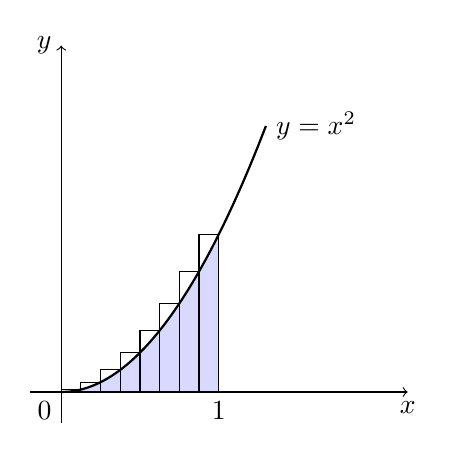
\begin{tikzpicture}[scale=2.0]
  % Axes
  \draw[->] (-0.2,0) -- (2.2,0) node[below] {$x$};
  \draw[->] (0,-0.2) -- (0,2.2) node[left] {$y$};
   \fill[blue!15] (1,0) -- plot[domain=0:1] (\x,{\x*\x}) -- (1,0) -- cycle;

  % a,b
  \draw (0,0) node[below left] {$0$} -- (0,0.1);
  \draw (1,0) node[below] {$1$}-- (1,1);
  % Partition points
  \def\xa{0}
  \def\xb{1}
  \def\n{8}
  \pgfmathsetmacro{\h}{(\xb-\xa)/\n}
  % Rectangles with right endpoints
  \foreach \k in {1,...,\n}{
    \pgfmathsetmacro{\xkm}{(\xa+(\k-1)*\h)}
    \pgfmathsetmacro{\xk}{\xa+\k*\h}
    \pgfmathsetmacro{\xkl}{\xa+(\k)*\h}
    \pgfmathsetmacro{\f}{\xkl*\xkl}
    \draw(\xkm,0) rectangle (\xk,\f);
    \draw[dashed] (\xk,0) -- (\xk,\f);
  }

  % Function
  \draw[domain=0:1.3,smooth,thick] plot(\x,\x*\x) node[right] {$y=x^2$};
\end{tikzpicture}
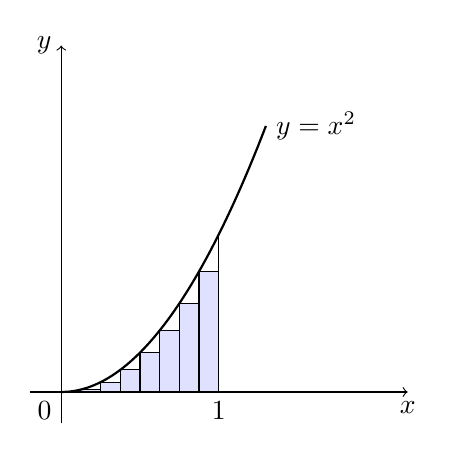
\begin{tikzpicture}[scale=2.0]
  % Axes
  \draw[->] (-0.2,0) -- (2.2,0) node[below] {$x$};
  \draw[->] (0,-0.2) -- (0,2.2) node[left] {$y$};
   

  % a,b
  \draw (0,0) node[below left] {$0$} -- (0,0.1);
  \draw (1,0) node[below] {$1$}-- (1,1);
  % Partition points
  \def\xa{0}
  \def\xb{1}
  \def\n{8}
  \pgfmathsetmacro{\h}{(\xb-\xa)/\n}
  % Rectangles with right endpoints
  \foreach \k in {1,...,\n}{
    \pgfmathsetmacro{\xkm}{(\xa+(\k-1)*\h)}
    \pgfmathsetmacro{\xk}{\xa+\k*\h}
    \pgfmathsetmacro{\xkl}{\xa+(\k-1)*\h}
    \pgfmathsetmacro{\f}{\xkl*\xkl}
    \draw[fill=blue!12](\xkm,0) rectangle (\xk,\f);
    \draw[dashed] (\xk,0) -- (\xk,\f);
  }

  % Function
  \draw[domain=0:1.3,smooth,thick] plot(\x,\x*\x) node[right] {$y=x^2$};
\end{tikzpicture}  
\end{center}
\end{example} 
\begin{example}[Тогтмол функцийн тодорхой интеграл: тодорхойлолтоор бодъё]
Дараах интегралыг \emph{тодорхойлолтын дагуу} (интеграл нийлбэр ашиглан) бодъё:
\[
\int_{2}^{5} 3\,dx.
\]

\textbf{Тодорхойлолт сануулъя.} \;
$f$ функц $[a,b]$ завсарт тодорхойлогдсон байг. Хэрэв
\[
\lim_{|P|\to 0} \sum_{k=1}^{n} f(\xi_k)\,\Delta x_k
\]
хязгаар оршин байвал, үүнийг $f$-ийн $[a,b]$ завсар дахь \emph{тодорхой интеграл} гээд
\[
\int_a^b f(x)\,dx
\]
гэж тэмдэглэнэ. Энд $\Delta x_k$ нь завсрын өргөн, $\xi_k$ нь $[x_{k-1},x_k]$ доторх дурын цэг. $P$ хуваалтын диаметр $|P|\to 0$ тул $n\to\infty$ байх нь тодорхой. Иймд хуваалтыг жигд (ижил урттай) хийвэл \[
\int_a^b f(x)\,dx=\lim_{n\to\infty} \sum_{k=1}^{n} f(\xi_k)\,\Delta x_k
\]
гэж болно.
\medskip

Манай жишээнд $f(x)=3$, $a=2$, $b=5$.

\textbf{1. Хуваалт авъя.} \;
$[2,5]$ завсрыг $n$ тэнцүү хэсэгт хуваая:
\[
\Delta x = \frac{5-2}{n} = \frac{3}{n}.
\]
Тэгвэл хуваалтын цэгүүд:
\[
x_k = 2 + k\Delta x = 2 + k\cdot\frac{3}{n},\quad k=0,1,\dots,n.
\]

\textbf{2. Дотоод цэг сонгоё.} \;
Сулралгүй байхын тулд баруун төгсгөлийг сонгоё:
\[
\xi_k = x_k = 2 + k\cdot\frac{3}{n},\quad k=1,2,\dots,n.
\]
(Тогтмол функцийн хувьд хаана сонгосон нь ялгаагүй.)

\textbf{3. Интеграл нийлбэр бичье.}
\[
S_n
=
\sum_{k=1}^{n} f(\xi_k)\,\Delta x
=
\sum_{k=1}^{n} 3\cdot\frac{3}{n}
=
\sum_{k=1}^{n} \frac{9}{n}
=
\frac{9}{n}\cdot n
=
9.
\]

\textbf{4. Хязгаар авч тодорхой интегралыг олъё.}
\[
\int_{2}^{5} 3\,dx
=
\lim_{n\to\infty} S_n
=
\lim_{n\to\infty} 9
=
9.
\]

\textbf{Дүгнэлт.}
\[
\boxed{\int_{2}^{5} 3\,dx = 9}
\]
гэж тодорхойлолтын дагуу (интеграл нийлбэрээр) бодож гаргалаа.

\medskip

Доорх зурагт $y=3$ шулуун ба $[2,5]$ завсрын хоорондох талбайг (өндөр $3$, суурь $3$ бүхий тэгш өнцөгт) үзүүлэв.

\begin{center}
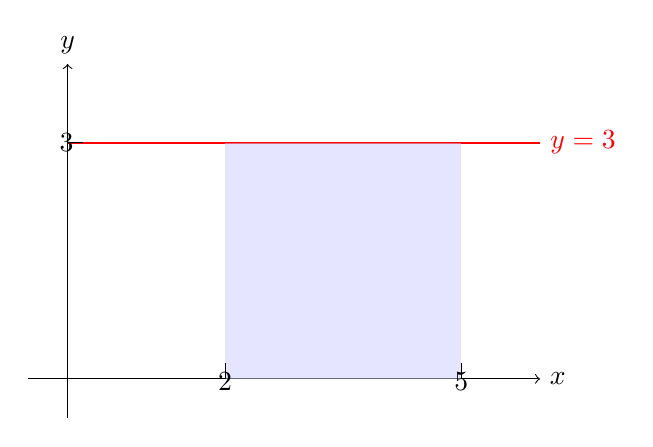
\begin{tikzpicture}[scale=1]
  % Axes
  \draw[->] (-0.5,0) -- (6,0) node[right] {$x$};
  \draw[->] (0,-0.5) -- (0,4) node[above] {$y$};

  % constant function
  \draw[thick,red] (0,3) -- (6,3) node[right] {$y=3$};

  % rectangle for integral
  \fill[blue!20,opacity=0.5] (2,0) rectangle (5,3);

  % x labels
  \draw (2,0) -- (2,0.2) node[below] {$2$};
  \draw (5,0) -- (5,0.2) node[below] {$5$};

  % y label
  \draw (0,3) -- (0.2,3) node[left] {$3$};
\end{tikzpicture}
\end{center}

\end{example}

\section{Тодорхой интегралын үндсэн чанарууд}

Доорх чанаруудыг интеграл нийлбэрийн тодорхойлолт ашиглан хялбар баталж болно.

\begin{theorem}[Тодорхой интегралын үндсэн чанарууд]
 $f,g$ функцүүд $[a,b]$ завсар дээр интегралчлагддаг байг.
\begin{enumerate}
\item \[
\int_a^a f(x)\,dx
=0
\]
    \item Шугаман чанар\\
аливаа тогтмол $\alpha,\beta$- хувьд $\alpha f(x)+\beta g(x)$ функц интегралчагдах бөгөөд
\[
\int_a^b (\alpha f(x)+\beta g(x))\,dx
=
\alpha\int_a^b f(x)\,dx + \beta\int_a^b g(x)\,dx.
\]
\item Аддитив чанар\\
Хэрэв $c$ нь $[a;b]$  завсрын ($a<b$) дурын цэг бол $y=f(x)$ функц $[a;c]$ ба $[c;b]$ завсарууд дээр интегралчлагдах ба 
\[
\int_a^b f(x)\,dx
=
\int_a^c f(x)\,dx + \int_c^b f(x)\,dx.
\]
\item Интеграл ба тэнцэтгэл биш \\
Хэрэв  $\forall x\in[a,b]$ хувьд $f(x)\ge 0$ бол
\[
\int_a^b f(x)\,dx \ge 0.
\]
Нэмэлтээр, хэрэв $\forall x\in[a,b]$ хувьд $f(x)\ge g(x)$  бол
\[
\int_a^b f(x)\,dx \ge \int_a^b g(x)\,dx.
\]
\item 
Хэрэв $\forall x\in[a,b]$ хувьд $m\le f(x)\le M$  бол
\[
m(b-a) \le \int_a^b f(x)\,dx \le M(b-a).
\]
\end{enumerate}
\end{theorem}
\begin{example} \[
\int_{-1}^{2} f(x)\,dx = 5, 
\qquad 
\int_{-1}^{2} g(x)\,dx = -3.
\] бол
  $\displaystyle\int_{-1}^{2}\bigl[f(x)+2g(x)\bigr]\,dx$–ийг тооцол.

Шугаман чанараар 
 $\displaystyle\int_{-1}^{2}\bigl[f(x)+2g(x)\bigr]\,dx=\displaystyle\int_{-1}^{2}f(x)\,dx+2\displaystyle\int_{-1}^{2}g(x)\,dx=5+2\cdot (-3)=-1.$
\end{example}
\begin{example}
\[
\int_{0}^{1} f(x)\,dx = -2,  
\qquad 
\int_{0}^{5} f(x)\,dx =1.
\] бол $\displaystyle\int_{1}^{5} f(x)\,dx$–ийг ол.\\
Аддитив чанараар $$\displaystyle\int_{0}^{5} f(x)\,dx=\displaystyle\int_{0}^{1} f(x)\,dx+\displaystyle\int_{1}^{5} f(x)\,dx$$ тул $\displaystyle\int_{1}^{5} f(x)\,dx=\displaystyle\int_{0}^{5} f(x)\,dx-\displaystyle\int_{0}^{1} f(x)\,dx=3.$

\end{example}
\section{Тодорхой интеграл ба уламжлал}
\begin{theorem}[Дифференциал тоололын үндсэн теорем I]
$f$ нь $[a,b]$ дээр тасралтгүй функц байг. 
\[
A(x)=\int_a^x f(t)\,dt \quad (a\le x\le b)
\]
гэж тодорхойлъё. Тэгвэл $A(x)$ нь $[a,b]$ дээр дифференциалчлагдах ба
\[
A'(x)=f(x)\quad (a<x<b).
\]
\end{theorem}

\begin{prof}
Ямар нэг тогтмол $x\in(a,b)$ авъя. $A'(x)$-ийг тодорхойлолтоор нь:
\[
A'(x)=\lim_{h\to0}\frac{A(x+h)-A(x)}{h}.
\]

Эхлээд $h\to 0$ тул $x+h\in[a,b]$ гэж үзэж болно. Тэгвэл аддитив чанараар
\[
A(x+h)-A(x)
= \int_a^{x+h} f(t)\,dt - \int_a^x f(t)\,dt
= \int_x^{x+h} f(t)\,dt.
\]
Иймээс
\[
\frac{A(x+h)-A(x)}{h}
=
\frac{1}{h}\int_x^{x+h} f(t)\,dt.
\]

Одоо $[x,x+h]$ завсар дээр $f$ тасралтгүй тул битүү завсар дээр хамгийн их ба бага утга авна. Иймээс
\[
m_h=\min_{t\in[x,x+h]} f(t),\qquad M_h=\max_{t\in[x,x+h]} f(t)
\]
тоонууд оршино.

Хялбар болгохын тулд $h>0$ тохиолдлыг эхэлж авч үзье. ( $h<0$ үед яг ижил аргаар бодно.) Тэгвэл интеграл ба тэнцэтгэл биш чанараар дараах тэнцэтгэл биш биелнэ:
\[
m_h\cdot h
\ \le\
\int_x^{x+h} f(t)\,dt
\ \le\
M_h\cdot h.
\]
\[
m_h \le f(t)\le M_h \quad (t\in[x,x+h]).
\]
Иймээс
\[
m_h\cdot h
\ \le\
\int_x^{x+h} f(t)\,dt
\ \le\
M_h\cdot h.
\]
$h>0$ тул $h$-д хуваагаад:
\[
m_h
\ \le\
\frac{1}{h}\int_x^{x+h} f(t)\,dt
\ \le\
M_h.
\]
Өөрөөр хэлбэл
\[
m_h
\ \le\
\frac{A(x+h)-A(x)}{h}
\ \le\
M_h.
\]

Одоо $h\to0$ үед юу болохыг харъя. $f$ нь $x$ дээр тасралтгүй тул
\[
\lim_{h\to0} m_h = f(x),\qquad \lim_{h\to0} M_h = f(x).
\]
Учир нь $h\to0$ үед $[x,x+h]$ (эсвэл $[x+h,x]$) завсар $x+h\to x$,   $f$ тасралтгүй учраас хамгийн бага, их утгууд нь $f(x)$ рүү дөхнө.
Хязгаар ба тэнцэтгэл биш чанараар :
\[
\lim_{h\to0}\frac{A(x+h)-A(x)}{h} = f(x).
\]
Үүний зүүн тал нь $A'(x)$-ийн тодорхойлолт тул
\[
A'(x)=f(x).
\]

$h<0$ тохиолдолд $[x+h,x]$ завсрыг авч яг ижил алхмуудтайгаар баталж болно. Иймээс бүхэлд нь $a<x<b$ завсар дээр $A'(x)=f(x)$ байна.
\end{prof}
\begin{theorem}[Ньютон--Лейбницийн томьёо]\label{N-L formula}
$f$ нь $[a,b]$ дээр тасралтгүй функц байг. $F$ нь $f$-ийн ямар нэг эх функц буюу
\[
F'(x)=f(x)
\quad(a\le x\le b)
\]
байдаг гэж үзье. Тэгвэл тодорхой интеграл
\[
\int_a^b f(x)\,dx = F(b)-F(a).
\]
\end{theorem}

\begin{prof}
Өмнөх теоремоор $\displaystyle A(x)=\int_a^x f(t)\,dt$ гэж тодорхойлбол $A'(x)=f(x)$.
Иймээс $A$ нь $f$-ийн нэг эх функц байна. $F$ нь мөн $f$-ийн эх функц тул 
\[
F'(x)=A'(x)
\quad\Rightarrow\quad
(F-A)'(x)=0.
\]
Иймээс $F(x)-A(x)=C$ тогтмол байна. Тэгэхээр
\[
F(x)=A(x)+C.
\]

Одоо $x=a$ гэж тавивал
\[
F(a)=A(a)+C = 0 + C,
\]
учир нь $A(a)=\displaystyle\int_a^a f(t)\,dt =0$. Тэгэхээр $C=F(a)$.

Иймээс
\[
F(b)=A(b)+F(a),
\qquad\Rightarrow\qquad
A(b)=F(b)-F(a).
\]

Харин $A(b)=\displaystyle\int_a^b f(t)\,dt$ тул 
\[
\int_a^b f(x)\,dx = F(b)-F(a).
\] батлагдана. Цаашид $F(b)-F(a)=F(x)\Big|_a^b$ гэж бичих болно.
\end{prof}
\begin{example}
\[
\int_0^2 (3x^2-4x+1)\,dx
=
\left(x^3-2x^2+x\right)\Big|_0^2
= (8-8+2)-(0)=2.
\]
\end{example}
Дээрх теорем \ref{N-L formula}-р $$\dfrac{\displaystyle\int_a^x f(t)\,dt}{dx}=f(x)$$ байна. 
\begin{example}
$f(x)=\dfrac{\sin x}{x}$ функц нь $x=0$ цэгийг агуулаагүй аливаа интервал дээр тасралтгүй байна. Иймд Ньютон–Лейбницийн теоремын дагуу $(0,+\infty)$ завсарт
\[
\frac{d}{dx}\left(\int_{1}^{x} \frac{\sin t}{t}\,dt\right)=\frac{\sin x}{x}.
\]

Өмнөх жишээнээс ялгаатай нь энэ интегралыг танил элементар функцүүдийн хувьд илэрхийлэн бодох боломжгүй. Иймээс энэхүү уламжлалыг олоход дээрх томьёо нь \textit{цорын ганц энгийн арга} юм.
\end{example}
\section{Тодорхой интегралд хэсэгчилж интегралчлах}

Тасралтгүй $f(x)$ ба $g(x)$ функцууд байг. Тэгвэл тодорхой интегралд 
хэсэгчилж интегралчлах томьёо нь
\[
\int_a^b f(x)g'(x)\,dx
=
\Bigl[f(x)g(x)\Bigr]_{x=a}^{x=b}-\int_a^b f'(x)g(x)\,dx .
\]
\begin{example}
\[
\int_0^1 x e^x\,dx
\]
 
\[
f(x)=x,\qquad f'(x)=1,\qquad g'(x)=e^x,\qquad g(x)=e^x
\] гэж сонговол
\[
\int_0^1 x e^x\,dx
=
\Bigl[x e^x\Bigr]_0^1-\int_0^1 e^x\,dx.
\]

\[
=
(e^1-0)-\bigl[e^x\bigr]_0^1
=
e-(e-1)=1.
\]

\[
\boxed{\displaystyle\int_0^1 x e^x\,dx=1.}
\]
\end{example}
\begin{example}
\[
\int_0^\pi x\sin x\,dx
\]
\[
f(x)=x,\qquad f'(x)=1,\qquad g'(x)=\sin x,\qquad g(x)=-\cos x.
\]
гэж сонговол
\[
\int_0^\pi x\sin x\,dx
=
\Bigl[-x\cos x\Bigr]_0^\pi
-
\int_0^\pi (-\cos x)\,dx.
\]

\[
=-\pi\cos\pi+0-\int_0^\pi (-\cos x)\,dx
=\pi+\int_0^\pi \cos x\,dx.
\]

\[
=\pi+\bigl[\sin x\bigr]_0^\pi
=\pi+(0-0)=\pi.
\]

\[
\boxed{\displaystyle\int_0^\pi x\sin x\,dx=\pi.}
\]
    
\end{example}
\section{Тодорхой интегралд орлуулалтын арга}

Хэрэв $\varphi$ нь $[a,b]$ дээр дифференциалчлагддаг, 
$f$ нь $\varphi(a)$ ба $\varphi(b)$--ийн хооронд тасралтгүй бол

\[
\int_a^b f(\varphi(x))\varphi'(x)\,dx
=
\int_{\varphi(a)}^{\varphi(b)} f(u)\,du.
\]
\begin{example}
\[
\int_0^1 2x\cos(x^2)\,dx.
\]

$\varphi(x)=x^2$ орлуулга хийе. \quad $u=\varphi(x)=x^2$ \;\; $\Rightarrow\; du=2x\,dx$.
Шинэ хил  
\[
x=0\Rightarrow u=\varphi(0)=0^2=0,\qquad x=1\Rightarrow u=\varphi(1)=1^2=1.
\]

\[
\int_0^1 2x\cos(x^2)\,dx
=
\int_0^1 \cos u\,du
=
\sin u\Big|_0^1
=\sin1-0=\sin1.
\]

\[
\boxed{\int_0^1 2x\cos(x^2)\,dx=\sin1.}
\]

\end{example}
\begin{example}
\[
\int_0^{\frac{\pi}{2}}\sin x\cos x\,dx.
\]

 $u=\sin x$  орлуулга хийвэл $\Rightarrow\; du=\cos x\,dx$.

Хил:
\[
x=0\Rightarrow u=0,\qquad x=\frac{\pi}{2}\Rightarrow u=1.
\]

\[
\int_0^{\frac{\pi}{2}}\sin x\cos x\,dx
=
\int_0^{1} u\,du
=
\frac{u^2}{2}\Big|_0^1
=\frac12.
\]

\[
\boxed{\displaystyle \int_0^{\frac{\pi}{2}}\sin x\cos x\,dx=\frac12.}
\]

\end{example}
\section{Семинар}
\begin{enumerate}
    \item Доорх функцуудын хувьд өгөгдсөн завсрыг 
$n=4$ адил урттай хуваагаад 
\[
\sum_{k=1}^4 f(x_k^*)\,\Delta x
\]
 нийлбэрийг тооцоол.
Энд $x_k^*$ нь дараах гурван тохиолдлоор авна:
\begin{enumerate}
\item[a)]  завсрын \textbf{зүүн} төгсгөл
\item[b)]  завсрын \textbf{дундаж} цэг
\item[c)]  завсрын \textbf{баруун} төгсгөл
\end{enumerate}

Бүх тохиолдолд график зурж, тухайн нийлбэрийг илэрхийлж буй тэгш өнцөгтүүдийн талбайг харуул.
\begin{enumerate}
\item $f(x)=3x+1$, \quad завсар: $[2,\,6]$

\item $f(x)=\frac{1}{x}$, \quad завсар: $[1,\,9]$

\item $f(x)=\cos x$, \quad завсар: $[0,\,\pi]$

\item $f(x)=2x-x^2$, \quad завсар: $[-1,\,3]$
\end{enumerate}
\item \[
f(x)=
\begin{cases}
|x-2|, & x\ge0,\\[4pt]
x+2, & x<0.
\end{cases}
\] бол дараах интегралуудыг ол.
\begin{enumerate}
\begin{multicols}{2}
\item $\displaystyle\int_{-2}^{0} f(x)\,dx$
\item $\displaystyle\int_{-2}^{2} f(x)\,dx$
\item $\displaystyle\int_{0}^{6} f(x)\,dx$
\item $\displaystyle\int_{-4}^{6} f(x)\,dx$  
\end{multicols}
\end{enumerate}
\item 
\[
f(x)=
\begin{cases}
2x, & x\le1,\\[4pt]
2, & x>1.
\end{cases}
\]
бол дараах интегралуудыг ол.
\begin{enumerate}
\begin{multicols}{2}
\item $\displaystyle\int_{0}^{1} f(x)\,dx$
\item $\displaystyle\int_{-1}^{1} f(x)\,dx$
\item $\displaystyle\int_{1}^{10} f(x)\,dx$
\item $\displaystyle\int_{1/2}^{5} f(x)\,dx$
\end{multicols}
\end{enumerate}
\item Доорх зураг нь $y=f(x)$ муруй ба $ox$ тэнхлэгийн хоорондох талбайн утгуудыг өгөв. Тэдгээрийг ашиглан 
$$
\int_a^b f(x)\,dx,\quad
\int_b^c f(x)\,dx,\quad
\int_a^c f(x)\,dx,\quad
\int_a^d f(x)\,dx
$$ интегралуудыг ол.
\begin{figure}[h]
\centering
\begin{tikzpicture}[scale=1.5]
  % axes
  \draw[->] (-0.2,0) -- (5.2,0) node[right]{$x$};
  \draw[->] (0,-1) -- (0,2) node[above]{$y$};

  % points a<b<c<d on x-axis
  \coordinate (A) at (0.5,0);
  \coordinate (B) at (1.5,0);
  \coordinate (C) at (2.8,0);
  \coordinate (D) at (4.5,0);

  \node[below] at (A) {$a$};
  \node[below] at (B) {$b$};
  \node[below] at (C) {$c$};
  \node[below] at (D) {$d$};

  % curve (just a smooth spline)
  \draw[thick,domain=0.3:4.7,smooth]
     plot(\x,{0.8*sin(120*\x)+0.3*\x-0.5});

  % shaded areas: [a,b] positive 0.8
  \fill[blue!20] (A) --
    plot[domain=0.5:1.5,smooth] (\x,{0.8*sin(120*\x)+0.3*\x-0.5}) --
    (B) -- cycle;
  \node at (1,0.6) {\small  талбай$=0.8$};

  % [b,c] negative 2.6
  \fill[cyan!25] (B) --
    plot[domain=1.5:3,smooth] (\x,{0.8*sin(120*\x)+0.3*\x-0.5}) --
    (C) -- cycle;
  \node at (2.2,-1) {\small талбай $=1$};

  % [c,d] positive 1.5
  \fill[red!20] (C) --
    plot[domain=3:4.5,smooth] (\x,{0.8*sin(120*\x)+0.3*\x-0.5}) --
    (D) -- cycle;
  \node at (3.8,1.2) {\small талбай $=1.6$};

  \node[right] at (4.7,1.8) {$y=f(x)$};
\end{tikzpicture}
\end{figure}

\item Дараах функцүүдийн график ба $ox$ тэнхлэгийн өгөгдсөн интервалаар хүрээлэгдсэн хэсгийн талбайг ол.
\begin{enumerate}
\begin{multicols}{2}
\item $f(x)=x^3,\quad [2,3]$
\item $f(x)=x^4,\quad [-1,1]$
\item $f(x)=3\sqrt{x},\quad [1,4]$
\item $f(x)=x^{-2/3},\quad [1,27]$
\item $f(x)=e^{2x},\quad [0,\ln2]$
\item $f(x)=\dfrac1x,\quad [1,5]$
\end{multicols}
\end{enumerate}

\item Дараах интегралуудыг Ньютон-Лейбницийн теоремийг ашиглан бод.

\begin{enumerate}
\begin{multicols}{2}
\item $\displaystyle\int_{-2}^{1}(x^2-6x+12)\,dx$
\item $\displaystyle\int_{-1}^{2}4x(1-x^2)\,dx$
\item $\displaystyle\int_{1}^{4}\frac{4}{x^2}\,dx$
\item $\displaystyle\int_{1}^{2}\frac1{x^6}\,dx$
\item $\displaystyle\int_{4}^{9}2x\sqrt{x}\,dx$
\item $\displaystyle\int_{1}^{4}\frac1{x\sqrt{x}}\,dx$
\item $\displaystyle\int_{-\pi/2}^{\pi/2}\sin\theta\,d\theta$
\item $\displaystyle\int_{0}^{\pi/4}\sec^2\theta\,d\theta$
\item $\displaystyle\int_{-\pi/4}^{\pi/4}\cos x\,dx$
\item $\displaystyle\int_{0}^{\pi/3}(2x-\sec x\tan x)\,dx$
\item $\displaystyle\int_{\ln2}^{3}5e^x\,dx$
\item $\displaystyle\int_{1/2}^{1}\frac1{2x}\,dx$
\item $\displaystyle\int_{-1}^{1}\frac1{1+x^2}\,dx$
\item $\displaystyle\int_{0}^{1/\sqrt2}\frac{dx}{\sqrt{1-x^2}}$
\item $\displaystyle\int_{\sqrt2}^{2}\frac{dx}{x\sqrt{x^2-1}}$
\item $\displaystyle\int_{-\sqrt3}^{-2/\sqrt3}\frac{dx}{x\sqrt{x^2-1}}$
\item $\displaystyle\int_{1}^{4}\left(\frac1{\sqrt t}-3\sqrt t\right)\,dt$
\item $\displaystyle\int_{\pi/6}^{\pi/2}\left(x+\frac2{\sin^2 x}\right)\,dx$
\end{multicols}
\end{enumerate}
\item Дараах интегралуудын уламжлалыг ол.
\begin{enumerate}
\begin{multicols}{2}
\item $\displaystyle \frac{d}{dx}\int_{1}^{x}\sin(t^2)\,dt$
\item $\displaystyle \frac{d}{dx}\int_{0}^{x} e^{\sqrt{t}}\,dt$
\item $\displaystyle \frac{d}{dx}\int_{0}^{x}\frac{dt}{1+\sqrt{t}}$
\item $\displaystyle \frac{d}{dx}\int_{1}^{x}\ln t\,dt$
\item $\displaystyle \frac{d}{dx}\int_{x}^{0} t\sec t\,dt$
\item $\displaystyle \frac{d}{du}\int_{0}^{u}|x|\,dx$
\end{multicols}
\end{enumerate}
\item $\displaystyle F(x)=\int_{4}^{x}\sqrt{t^2+9}\,dt$ бол\qquad 
 $
\text{(a) }F(4),\qquad \text{(b) } F'(4),\qquad \text{(c) }F''(4)$ ол.
\item Тодорхой интегралыг орлуулах аргаар бод.
\begin{enumerate}
 \begin{multicols}{2}
\item $\displaystyle \int_{0}^{1}(2x+1)^3\,dx$
\item $\displaystyle \int_{1}^{2}(4x-2)^3\,dx$
\item $\displaystyle \int_{0}^{1}(2x-1)^3\,dx$
\item $\displaystyle \int_{1}^{2}(4-3x)^8\,dx$
\item $\displaystyle \int_{0}^{8}x\sqrt{1+x}\,dx$
\item $\displaystyle \int_{-3}^{0}x\sqrt{1-x}\,dx$
\item $\displaystyle \int_{0}^{\pi/2}4\sin\frac{x}{2}\,dx$
\item $\displaystyle \int_{0}^{\pi/6}2\cos3x\,dx$
\item $\displaystyle \int_{-2}^{-1}\frac{x}{(x^2+2)^3}\,dx$
\item $\displaystyle \int_{1-\pi}^{1+\pi}\sec^2\!\Bigl(\frac14 x-\frac14\Bigr)\,dx$
\item $\displaystyle \int_{-\ln3}^{\ln3}\frac{e^{x}}{e^x+4}\,dx$
\item $\displaystyle \int_{0}^{\ln5}e^{x}(3-4e^x)\,dx$
\item $\displaystyle \int_{1}^{3}\frac{dx}{\sqrt{x}(x+1)}$
\item $\displaystyle \int_{\ln2}^{\ln(2/\sqrt3)}
       \frac{e^{-x}\,dx}{\sqrt{\,1-e^{-2x}\,}}$
\end{multicols}
\end{enumerate}
\item Тодорхой интегралыг хэсэгчлэх аргаар бод.
\begin{enumerate}
\begin{multicols}{2}
\item $\displaystyle \int_{0}^{\ln2} x e^{-x}\,dx$
\item $\displaystyle \int_{0}^{\pi} x\sin x\,dx$
\item $\displaystyle \int_{0}^{2\pi} x^3\cos x\,dx$
\item $\displaystyle \int_{1/e}^{e} |\ln x|\,dx$
\item $\displaystyle \int_{0}^{\sqrt3} x\arctan x\,dx$
\item $\displaystyle \int_{0}^{\pi} e^x\sin x\,dx$
\end{multicols}
\end{enumerate}
\item  Интегралыг бод.
\begin{multicols}{2}
\begin{enumerate}
  \item $\displaystyle \int_{0}^{1} x\,(2-x^{2})^{18}\,dx$.

  \item $\displaystyle \int_{-1}^{1} \frac{x\,dx}{x^{2}+x+1}$.

  \item $\displaystyle \int (x\ln x)^{2}\,dx$.

  \item $\displaystyle \int_{0}^{9} x^{3}\sqrt[3]{1-x}\,dx$.

  \item $\displaystyle \int_{-2}^{-1} \frac{dx}{x\sqrt{x^{2}-1}}$.

  \item $\displaystyle \int_{1/2}^{1} x^{16}\sqrt{1+3x^{8}}\,dx$.

  \item $\displaystyle \int_{0}^{3} \arcsin\sqrt{\frac{x}{1+x}}\,dx$.

  \item $\displaystyle \int_{0}^{2\pi} \frac{dx}{(2+\cos x)(3+\cos x)}$.

  \item $\displaystyle \int_{0}^{2\pi} \frac{dx}{\sin^{4}x+\cos^{4}x}$.

  \item $\displaystyle \int_{0}^{\pi/2} \sin x\,\sin 2x\,\sin 3x\,dx$.

  \item $\displaystyle \int_{0}^{\pi} (x\sin x)^{2}\,dx$.

  \item $\displaystyle \int_{0}^{\pi} e^{x}\cos^{3}x\,dx$.

  \item $\displaystyle \int_{0}^{\ln 2} \sinh^{4}x\,dx$.
\end{enumerate}
    
\end{multicols}
\end{enumerate}
